\documentclass[a4paper]{article}
\usepackage{hyperref}
\usepackage{graphicx}
\graphicspath{ {./} }
\usepackage[utf8]{inputenc}

\title{Pandit Extended Abstract}
\author{Eric Gerard Moynihan}
\date{March 2022}

\begin{document}

\maketitle

\section{Introduction}
Pandit at its core is a \textbf{distributed service-level proxy}.
This means it is a proxy tasked with interpreting data on a service level and caching it
in a distributed manner, allowing it to speed up read and write times of clients querying the services
in question.

Pandit is designed to be able to proxy any data source such as REST APIs or SQL databases.
It reads in user-defined Protocol Buffers \cite{protobufs} that are extended to provide information on
how to parse, cache, and return data to clients.

It uses these Protobufs to provide a gRPC \cite{grpc} service that will be available to every client of every node.


\section{Existing Solutions}
Service level proxies usually fall into two categories:
\begin{itemize}
    \item A commercial closed-source proxy that focuses on platform-specific use cases.
    \item An open-source proxy that proxies requests and caches the responses.
\end{itemize}
\subsection{Commercial Closed-Source Proxies}
An example of the former would be Google Cloud Endpoints with HTTP/JSON to gRPC encoding \cite{cloud_endpoints}.
This feature exists in Pandit and functions similarly - as in it provides a conversion layer between
HTTP/JSON and gRPC. However, Google Cloud Endpoints only support a single data format (HTTP/JSON), while Pandit supports
many more data formats.
This form of proxy only works on the hosted Google Cloud Platform \cite{google_cloud_platform} while Pandit can be deployed
in any cluster.

\subsection{Open-Source Proxies}
Envoy Proxy \cite{envoy} is an example of an open-source proxy that is used to proxy requests and cache the responses.
Like Pandit, it supports many data formats and can be deployed in any cluster.
It runs alongside each application in the cluster and handles the querying and caching of data.
Pandit has a similar approach to this, with one key difference - Pandit provides a gRPC service to the clients.

The benefit of translating data to Protocol Buffers to be transferred over gRPC are numerous:
\begin{itemize}
    \item Clients can take advantage of code generation based on the Proto specification. \cite{codegen}
    \item Protocol Buffers are a binary format and hence more space-efficient than text-based formats such as JSON. \cite{encoding}
    \item gRPC benefits from features of HTTP/2 such as pipelining and compression. \cite{http2}
\end{itemize}

Since the cached data will also be stored in the Protocol Buffer format, it also means that cached data will be more space-efficient in
many cases.

Pandit is aware of all clients that have previously queried an endpoint and can sync the cache with the local daemon on each host the
clients are running on.
This means that the data will be widely available close to the clients and when it sees a query for the same data, it will return the cached data.
Users of course define if and how long the data should be cached, as well as how to recognise a query for the same data.

All these features mean Pandit provides a great deal of flexibility for users to define their own caching and querying strategies.

\section{Implementation}
\subsection{UML Diagram}
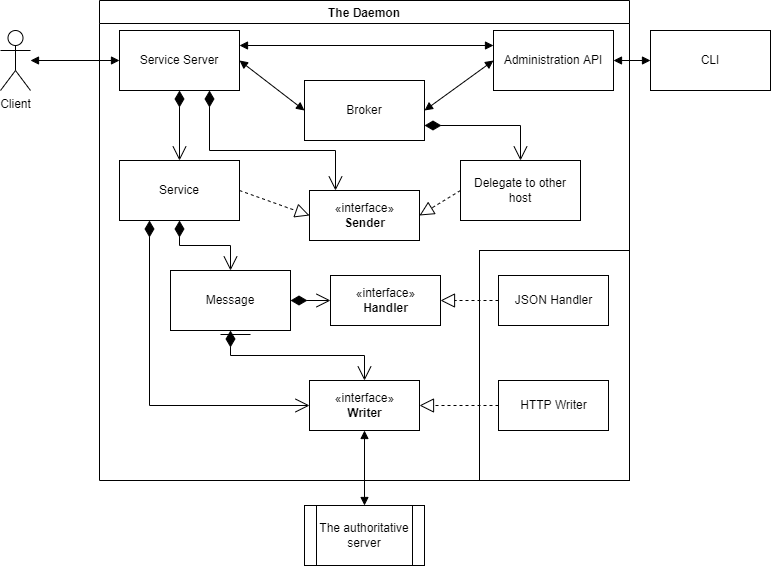
\includegraphics[scale=0.45]{uml}
\subsection{Overview}
A single instance of the Pandit daemon will be run on each host in a cluster of machines. When a client queries
a service, the daemon will first check the cache for the data. If it cannot find it, it will delegate the request
to an authoritative container in the cluster.

Since the mapping between the data returned by the authoritative container and the data returned by the gRPC service is
user-defined, Pandit provides options to annotate specific fields in return types to allow for the efficient caching of
common requests, greatly reducing the amount of queries that need to be sent to the authoritative container.

The entire project is implemented using the Rust Programming Language \cite{rust}, providing fast run times, compile-time memory safety
and top-notch tooling.

The daemon was implemented with the following features:

\subsection{Handler}
\label{sec:handler}
The \textit{\nameref{sec:handler}} is used to convert to and from the abstract fields representation of the data provided to the writer.

\subsection{Writer}
\label{sec:writer}
This is a trait \cite{trait} that represents a way of sending a query to the authoritative container.
It takes in the an abstract representation of the query data and a \textit{\nameref{sec:handler}}.
The writer uses the \textit{\nameref{sec:handler}} to convert the data to a bytes array.
It then constructs a full request in the format required with the payload from the handler.
Finally, it then sends the request to the authoritative container.

A current implementation of this is the HTTP Writer that uses a JSON handler to interface with REST APIs.

\subsection{Messages}
\label{sec:messages}
This represents a Protocol Buffer Message. A Method is defined by an input Message and an Output Message and so it will contain two instances of this struct.
A message contains many fields of different types, one of those types being another message. The message struct also contains all the
aforementioned information provided by the user in the Protobuf specification.

It provides methods that parse Protobuf encoded messages to and from an abstract representation of the fields and their values. This conversion has been
implemented mostly from scratch due to the unique requirement of parsing based on a specification provided on runtime. Most libraries utilise code generation
to provide server and client side parsing and so they were not suitable for use in this project.

\subsection{Service}
\label{sec:service}
This is a \textit{struct} that represents a service that is hosted by the daemon. It is created by the \textit{\nameref{sec:api}} and
takes in a Protobuf specification.

The constructor parses the Protobuf specification and builds an in-memory mapping of all methods, messages, and their fields.
This includes parsing user defined options for caching, such as the \textit{Primary Key} field that will define when a cache hit should occur.
Other options include the \textit{Cache Disabled} and \textit{Cache Timeout} fields that define if and how long the data should be cached.

The service provides a method that sends a query to the authoritative container on the host.
It passes the query as well as a \textit{\nameref{sec:handler}} for the specific method to a \textit{\nameref{sec:writer}} which executes the query
and returns the response. The response is then converted to a Protocol Buffer using the aforementioned \textit{\nameref{sec:handler}} and returned.

\subsection{Broker}
\label{sec:broker}

This is the glue that allows the daemon to be aware of and communicate with other daemons in the cluster.
The broker interfaces with a Redis \cite{redis} instance that is connected to all the daemons to facilitate this.

When constructing the broker, the user provides the address of the Redis instance which it will use it will maintain a connection to the Redis instance for the entirety of the run time.
It provides many methods to interact with the Redis instance:
\begin{itemize}
    \item To add a new \textit{\nameref{sec:service}} to the broker.
    \item To query the broker for the address of a \textit{\nameref{sec:service}}.
    \item To publish new cache to all interested daemons in the cluster.
    \item To check if cache exists for a specific query.
\end{itemize}

\subsection{Administration API}
\label{sec:api}
This is the API that is used to configure the daemon. It is a gRPC service that is exposed via a port on the loopback interface of each host.
A CLI client is used to interface with the API. Currently, the only supported method is to add a new \textit{\nameref{sec:service}} to the daemon.
This entails the following:
\begin{itemize}
    \item Creating a new \textit{\nameref{sec:service}} based on the parameters provided by the user.
          This includes providing Protobuf that was sent from the client as a byte array.
    \item Adding the service to the \textit{\nameref{sec:broker}}. This tells the other daemons about the service that this
          node is hosting the service in question.
\end{itemize}

\subsection{Service Server}
\label{sec:server}
This provides a custom gRPC service handler. It is responsible for handling all requests from clients on the host it's running on.
When a gRPC request is received, it will parse the service and method name from the request.
It will first check the cache for the data based on this information. If it cannot find it,
it will delegate the request to the \textit{\nameref{sec:service}}.

However, the \textit{\nameref{sec:service}} may not be available on the current host. In this case, the request will be delegated to the host that the
service is available on. The host is found by querying the \textit{\nameref{sec:broker}} for the address of the host the service is on.
After a response is received, it will publish the data to the cache using the \textit{\nameref{sec:broker}}.

\section{The CLI}
\label{sec:cli}
The CLI was implemented using the Rust programming language \cite{rust}.
It provides a command line interface to configure the daemon.
It imports the gRPC client library that was generated by the Protobuf compiler and uses it to interface with the daemon's \textit{\nameref{sec:api}}.
It currently is implemented to add a new \textit{\nameref{sec:service}} to the daemon by reading in a Protobuf specification from a file.

\section{Testing}
\subsection{Unit Testing}
Many unit tests were implemented to test the functionality of the the components of the daemon.
For example, the \textit{\nameref{sec:messages}} methods used to parse Protobuf payloads were tested to ensure that they provided the correct
data to the rest of the program.

The \textit{\nameref{sec:service}} was also tested to ensure that it called a \textit{\nameref{sec:writer}} when a query was made.

\subsection{Integration Testing}
In order to ensure the daemon was working correctly, a fake REST API was implemented in python to serve as an authoritative container.
A Protobuf specification was created for the API and it was passed to the daemon via \textit{\nameref{sec:cli}}.

The Protobuf specification was used to generate a Rust client library \cite{codegen} that was used to interact with the daemon.
A standalone testing binary was implemented by importing this library and calling the service in question.
It sent the same query twice, the first time it was ensured that the data came directly from the authoritative container, and the second time it was
ensured that the data came from the cache.

\section{Conclusion}
\textit{Pandit} is a great tool for caching and querying data in a distributed system.
It also provides a great deal of flexibility for users to define their own caching and querying strategies.

Whether it be a REST API or an SQL Database, all it takes is a single Protobuf specification \cite{protobufs} to turn it into a
\textbf{widely available gRPC \cite{grpc} Service}. Services become widely available due to the caching mechanism in the daemon being on every host,
as well as the publish/subscribe mechanism used to distribute the cache to all interested daemons.

The fact that anything can be turned into a gRPC service provides a lot more flexibility to the users of the product compared to any existing solution.
This is because you can build a client library for any language or framework using a Protobuf \cite{codegen}.

This also means that Pandit has innate benefits for any application that requires data from other services.
For example, instead of using an ORM \cite{orm} and manually encoding the data to be read in the application, you can use Pandit to
to turn the database into a gRPC service and then use the gRPC client library to read the data. This will give you the added benefit of
being able to cache the data and query it in a distributed system if it needs to be deployed to multiple hosts later on.
You could also implement another client in a different language in one step by generating code from the Protobuf \cite{codegen}.

Pandit also requires no configuration of the application being proxied. As long as pandit has the service added, it will be ready to accept requests.
This is because the daemon interfaces with the application as a client.

All-in-all, Pandit provides many benefits and the configuration process is both simple and intuitive.

\begin{thebibliography}{9}
    \bibitem{protobufs}
    Profocol Buffers documentation - \href{https://developers.google.com/protocol-buffers}{developers.google.com}.
    \bibitem{grpc}
    gRPC documentation - \href{https://grpc.io/docs/}{grpc.io}.
    \bibitem{cloud_endpoints}
    Google Cloud Endpoints Transcoding HTTP JSON to gRPC - \href{https://cloud.google.com/endpoints/docs/grpc/transcoding}{cloud.google.com}.
    \bibitem{google_cloud_platform}
    Google Cloud Platform - \href{https://cloud.google.com/}{cloud.google.com}.
    \bibitem{envoy}
    Envoy Proxy - \href{https://www.envoyproxy.io/docs/envoy/latest/intro/arch_overview/arch_overview}{envoyproxy.io}.
    \bibitem{codegen}
    Profocol Buffer Code Generation - \href{https://developers.google.com/protocol-buffers/docs/reference/go-generated}{developers.google.com}.
    \bibitem{encoding}
    Protocol Buffers Encoding - \href{https://developers.google.com/protocol-buffers/docs/encoding}{developers.google.com}.
    \bibitem{http2}
    HTTP 2 - \href{https://developer.mozilla.org/en-US/docs/Glossary/HTTP_2}{developer.mozilla.org}.
    \bibitem{rust}
    Rust Programming Language - \href{https://www.rust-lang.org/}{rust-lang.org}.
    \bibitem{core}
    gRPC Core Concepts - \href{https://grpc.io/docs/what-is-grpc/core-concepts/}{grpc.io}.
    \bibitem{redis}
    Redis - \href{https://redis.io/}{redis.io}.
    \bibitem{trait}
    Rust Traits - \href{https://doc.rust-lang.org/rust-by-example/trait.html}{doc.rust-lang.org}.
    \bibitem{orm}
    Object Relational Mapping - \href{https://en.wikipedia.org/wiki/Object%E2%80%93relational_mapping}{en.wikipedia.org}.
\end{thebibliography}

\end{document}